\documentclass[aspectratio=169, 10pt]{beamer}

% =============================================================
% 1. TEMA & KONFIGURASI VISUAL BEAMER (Gaya Template UNAIR)
% =============================================================
\mode<presentation> {
	\usetheme{Madrid}
	\useinnertheme{circles}
}

\usepackage{graphicx}
\usepackage{grffile}
\usepackage{booktabs}
\usepackage{mathtools}
\usepackage{amsmath,amssymb}
\usepackage{bm}
\usepackage{siunitx}
\usepackage{tabularx}
\usepackage{array}
\usepackage{tikz}
\usetikzlibrary{shapes.geometric,arrows.meta,positioning,fit,backgrounds}

% Direktori penyimpanan gambar
\graphicspath{{figures/}}

% Tipografi Font Charter & Professional Fonts
\usepackage{charter}
\usefonttheme{professionalfonts}

% ================= SIUNITX =================
\sisetup{output-decimal-marker={,}, per-mode=symbol}
\DeclareSIUnit\barn{barn}

% ================= WARNA RESMI UNAIR =================
\definecolor{UnairBlue}{HTML}{174B89}
\definecolor{UnairYellow}{HTML}{FFCC00}
\definecolor{DarkSlate}{HTML}{2C3E50}
\definecolor{CrimsonAlert}{HTML}{C0392B}
\definecolor{ForestGreen}{HTML}{27AE60}

\setbeamercolor{palette primary}{bg=UnairBlue,fg=white}
\setbeamercolor{palette secondary}{bg=UnairYellow,fg=UnairBlue}
\setbeamercolor{palette tertiary}{bg=UnairBlue,fg=white}
\setbeamercolor{palette quaternary}{bg=UnairBlue,fg=white}
\setbeamercolor{structure}{fg=UnairBlue}
\setbeamercolor{section in toc}{fg=UnairBlue}

% Warna Lingkungan Blok
\setbeamercolor{block title}{bg=UnairBlue,fg=white}
\setbeamercolor{block body}{bg=UnairBlue!8,fg=black}
\setbeamercolor{block title example}{bg=ForestGreen,fg=white}
\setbeamercolor{block body example}{bg=ForestGreen!8,fg=black}
\setbeamercolor{block title alert}{bg=CrimsonAlert,fg=white}
\setbeamercolor{block body alert}{bg=CrimsonAlert!8,fg=black}

% Font style
\setbeamerfont{title}{series=\bfseries,parent=structure}
\setbeamerfont{frametitle}{series=\bfseries,parent=structure}

% Nonaktifkan navigation symbols
\setbeamertemplate{navigation symbols}{}

% ================= HEADER FRAME DENGAN LOGO UNAIR =================
\setbeamertemplate{frametitle}{
	\vspace{-0.03cm}
	\begin{beamercolorbox}[
		wd=\paperwidth,
		ht=3.2ex,
		dp=1.1ex,
		leftskip=0.6em,
		rightskip=0.4em
		]{frametitle}
		\hbox to 0.97\paperwidth{
			\large\insertframetitle
			\hfill
			\raisebox{-0.18\height}{
\includegraphics[height=0.75cm]{logo-unair.png}}
		}
	\end{beamercolorbox}
}

% ================= FOOTLINE INFORMATIF TIGA BILAH =================
\setbeamertemplate{footline}{
	\leavevmode%
	\hbox{%
		\begin{beamercolorbox}[wd=.333333\paperwidth,ht=2.4ex,dp=1ex,center]{palette primary}%
			\textbf{\insertshortauthor}
		\end{beamercolorbox}%
		\begin{beamercolorbox}[wd=.333333\paperwidth,ht=2.4ex,dp=1ex,center]{palette secondary}%
			\textbf{\insertshorttitle}
		\end{beamercolorbox}%
		\begin{beamercolorbox}[wd=.333333\paperwidth,ht=2.4ex,dp=1ex,right]{palette primary}%
			\insertshortdate{}\hspace*{2em}
			\insertframenumber{} / \inserttotalframenumber\hspace*{2ex}
		\end{beamercolorbox}%
	}
	\vskip0pt
}

% ================= DATA PRESENTASI =================
\title[Resonansi $^{12}$C Breit-Wigner]{FITTING RESONANSI HAMBURAN NEUTRON\\$^{12}\text{C}(n,\text{tot})$ MODEL BREIT-WIGNER\\MENGGUNAKAN NEWTON-RAPHSON MULTIVARIAT}
\subtitle{Laporan Praktikum Fisika Komputasi II --- Studi Kasus 8}
\author[Kelompok H / Fisika Komputasi II]{
	Airin Khairunnisa Nur Raerah (182241045) \\
	Hendra Maulana (182241043)
}
\institute[UNAIR]{
	Departemen Fisika, Fakultas Sains dan Teknologi, Universitas Airlangga \\
	\medskip
	\textit{Laboratorium Fisika Komputasi}
}
\date[September 2026]{Surabaya, 12 September 2026}


% =============================================================
% DOKUMEN PRESENTASI
% =============================================================
\begin{document}

% -------------------------------------------------------------
% SLIDE 1: HALAMAN JUDUL
% -------------------------------------------------------------
\begin{frame}[plain]
	\titlepage
\end{frame}

% -------------------------------------------------------------
% SLIDE 2: DAFTAR ISI (OUTLINE)
% -------------------------------------------------------------
\begin{frame}{Daftar Isi Presentasi}
	\tableofcontents
\end{frame}


% =============================================================
% SECTION 1: TUJUAN & LATAR BELAKANG
% =============================================================
\section{Tujuan dan Latar Belakang Fisis}

% SLIDE 3
\begin{frame}{Latar Belakang: Resonansi Hamburan Neutron $^{12}$C}
	\begin{columns}[T]
		\begin{column}{0.52\textwidth}
			\begin{block}{Fenomena Fisis: Inti Majemuk $^{13}$C$^*$}
				\small
				\begin{itemize}
					\item Neutron dengan energi $1.8 \le E \le 2.4\text{ MeV}$ menumbuk inti $^{12}$C, membentuk inti majemuk $^{13}$C$^*$ pada keadaan eksitasi gelombang-D ($J^\pi = 5/2^+$).
					\item Terjadi lonjakan tajam penampang lintang total $\sigma(E)$ di sekitar energi resonansi $E_r \approx 2.078\text{ MeV}$.
					\item Data eksperimen dari IAEA-NDS EXFOR (Cierjacks et al., 1968): 59 titik observasi presisi tinggi.
				\end{itemize}
			\end{block}
		\end{column}

		\begin{column}{0.48\textwidth}
			\begin{alertblock}{Tantangan Komputasi Numerik}
				\small
				\begin{itemize}
					\item Model Breit-Wigner \textbf{non-linear} terhadap 4 parameter: $[E_r, \Gamma, \sigma_0, \sigma_{bg}]$.
					\item Regresi linier analitik tidak dapat diterapkan langsung.
					\item Diperlukan optimasi kelengkungan kuadratik berbasis \textbf{Newton-Raphson Multivariat} yang stabil dan presisi.
				\end{itemize}
			\end{alertblock}
		\end{column}
	\end{columns}
\end{frame}

% SLIDE 4
\begin{frame}{Tujuan Praktikum (Studi Kasus 8)}
	\begin{block}{7 Tujuan Komputasi yang Dicapai}
		\footnotesize
		\begin{enumerate}
			\item Memahami formulasi model resonansi satu tingkat Breit-Wigner secara matematis dan fisis.
			\item Menurunkan vektor gradien analitik $\mathbf{g}(\mathbf{p})$ dan matriks Hessian Gauss-Newton $\mathbf{H}(\mathbf{p}) = 2\mathbf{J}^T\mathbf{W}\mathbf{J}$.
			\item Mengimplementasikan solver Newton-Raphson multivariat $\mathbf{H}\Delta\mathbf{p} = -\mathbf{g}$ berbasis Python/NumPy.
			\item Mengekstrak parameter resonansi optimal $[E_r, \Gamma, \sigma_0, \sigma_{bg}]$ dari data IAEA-NDS EXFOR.
			\item Mengevaluasi kelayakan statistik model: $\chi^2_{red}$, matriks kovariansi $\mathbf{C}$, dan korelasi silang $\boldsymbol{\rho}$.
			\item Menguji ketahanan numerik melalui simulasi Monte Carlo \textit{noise stress-test} ($\eta = 5\%, 15\%, 30\%$).
			\item Memvalidasi hasil komputasi terhadap standar internasional ENDF/B-VIII.0 CIELO.
		\end{enumerate}
	\end{block}
\end{frame}


% =============================================================
% SECTION 2: DASAR TEORI
% =============================================================
\section{Landasan Teori}

% SLIDE 5
\begin{frame}{Model Breit-Wigner Satu Tingkat (\textit{Single-Level})}
	\begin{columns}[T]
		\begin{column}{0.5\textwidth}
			\begin{block}{Formula Penampang Lintang Resonansi}
				\small
				Penampang lintang total sebagai fungsi energi neutron $E$:
				\begin{equation}
					\sigma(E; \mathbf{p}) = \sigma_{bg} + \sigma_0 \frac{(\Gamma/2)^2}{(E - E_r)^2 + (\Gamma/2)^2}
				\end{equation}
				\footnotesize
				Profil Lorentzian simetris berpusat di $E_r$ dengan lebar penuh $\Gamma$ (FWHM). Vektor parameter 4-dimensi:
				\begin{equation}
					\mathbf{p} = [E_r,\; \Gamma,\; \sigma_0,\; \sigma_{bg}]^T
				\end{equation}
			\end{block}
		\end{column}

		\begin{column}{0.5\textwidth}
			\begin{exampleblock}{Fungsi Objektif Kuadrat Terkecil Terbobot}
				\small
				Minimasi $\chi^2$ terhadap $N = 59$ titik data:
				\begin{equation}
					\chi^2(\mathbf{p}) = \sum_{i=1}^{N} \frac{\left[\sigma_i - \sigma(E_i;\mathbf{p})\right]^2}{(\Delta\sigma_i)^2}
				\end{equation}
				\footnotesize
				Bobot $w_i = (\Delta\sigma_i)^{-2}$ memperhitungkan ketidakpastian eksperimen. Kondisi minimum: $\nabla_{\mathbf{p}} \chi^2 = \mathbf{g}(\mathbf{p}) = \mathbf{0}$.
			\end{exampleblock}
		\end{column}
	\end{columns}
\end{frame}

% SLIDE 6
\begin{frame}{Gradien Analitik \& Matriks Hessian Gauss-Newton}
	\begin{columns}[T]
		\begin{column}{0.5\textwidth}
			\begin{block}{Vektor Gradien $\mathbf{g}(\mathbf{p})$}
				\small
				\begin{equation}
					\mathbf{g}(\mathbf{p}) = -2\mathbf{J}^T\mathbf{W}\mathbf{r}
				\end{equation}
				\footnotesize
				dengan $\mathbf{r} = [\sigma_i - \sigma(E_i;\mathbf{p})]$ vektor residu, $\mathbf{W} = \mathrm{diag}(w_i)$ matriks bobot diagonal, dan $\mathbf{J}$ matriks Jacobian $(N\times 4)$:
				\begin{equation*}
					J_{ij} = \frac{\partial\sigma(E_i;\mathbf{p})}{\partial p_j}
				\end{equation*}
			\end{block}
		\end{column}

		\begin{column}{0.5\textwidth}
			\begin{alertblock}{Matriks Hessian Gauss-Newton $\mathbf{H}(\mathbf{p})$}
				\small
				Aproksimasi kelengkungan kuadratik yang selalu positif-semidefnit:
				\begin{equation}
					\mathbf{H}(\mathbf{p}) \approx 2\mathbf{J}^T\mathbf{W}\mathbf{J}
				\end{equation}
				\footnotesize
				\begin{itemize}
					\item Selalu simetris dan positif semi-definit: $\lambda_j \ge 0$.
					\item Tidak memerlukan diferensiasi orde kedua eksplisit.
					\item Jaminan arah langkah selalu menuruni $\chi^2$.
				\end{itemize}
			\end{alertblock}
		\end{column}
	\end{columns}
\end{frame}

% SLIDE 7
\begin{frame}{Algoritma Newton-Raphson Multivariat}
	\begin{columns}[T]
		\begin{column}{0.5\textwidth}
			\begin{block}{Persamaan Update Iteratif}
				\small
				Setiap langkah iterasi ke-$(k+1)$ menyelesaikan sistem linear:
				\begin{equation}
					\mathbf{H}(\mathbf{p}^{(k)})\,\Delta\mathbf{p} = -\mathbf{g}(\mathbf{p}^{(k)})
				\end{equation}
				\begin{equation}
					\mathbf{p}^{(k+1)} = \mathbf{p}^{(k)} + \Delta\mathbf{p}
				\end{equation}
				\footnotesize
				Diselesaikan via dekomposisi $LU$ (rutin \texttt{numpy.linalg.solve}, backend LAPACK \texttt{DGESV}).
			\end{block}
		\end{column}

		\begin{column}{0.5\textwidth}
			\begin{exampleblock}{Kriteria Konvergensi Ganda \& Kestabilan}
				\small
				Iterasi berhenti jika \textbf{salah satu} terpenuhi:
				\begin{equation*}
					\|\Delta\mathbf{p}\|_2 < \varepsilon = 10^{-6} \quad \text{atau} \quad |\Delta\chi^2| < \varepsilon
				\end{equation*}
				\footnotesize
				Laju konvergensi bersifat \textbf{kuadratik orde-dua} (jauh lebih cepat dari metode orde-satu \textit{Gradient Descent}). Pemantauan bilangan kondisi:
				\begin{equation*}
					\kappa(\mathbf{H}) = \frac{\lambda_{\max}}{\lambda_{\min}} < 10^{15}
				\end{equation*}
			\end{exampleblock}
		\end{column}
	\end{columns}
\end{frame}


% =============================================================
% SECTION 3: PIPELINE KOMPUTASI
% =============================================================
\section{Arsitektur Pipeline Komputasi}

% SLIDE 8 — TikZ Horizontal Flowchart
\begin{frame}{Pipeline Komputasi Numerik 7 Tahap}
\tikzset{
	stageBox/.style={
		draw=UnairBlue, fill=UnairBlue!12, line width=0.8pt,
		rounded corners=3pt,
		minimum width=1.85cm, minimum height=1.55cm,
		text width=1.75cm, align=center, font=\fontsize{5.5pt}{6.8pt}\selectfont
	},
	stepArrow/.style={
		-{Stealth[length=4pt,width=3.5pt]},
		draw=UnairYellow!80!orange, line width=1.4pt
	},
	startEnd/.style={
		draw=DarkSlate, fill=DarkSlate!15, line width=0.8pt,
		ellipse, minimum width=1.4cm, minimum height=0.7cm,
		text width=1.3cm, align=center, font=\fontsize{5pt}{6pt}\selectfont\bfseries
	},
	stageLabel/.style={
		font=\fontsize{5pt}{6pt}\selectfont\bfseries\color{UnairBlue},
		above=2pt
	}
}
\begin{center}
\begin{tikzpicture}[node distance=0.38cm and 0.30cm]

% ---- START node
\node[startEnd] (start) {MULAI\\[1pt]Data EXFOR};

% ---- Tahap 1
\node[stageBox, right=0.30cm of start] (t1)
	{\textbf{\color{UnairBlue}Tahap 1}\\[2pt]
	 Akuisisi Data\\IAEA-NDS EXFOR\\Entry 10224002\\
	 \textit{Parser ASCII}\\CSV ($N{=}59$)};

% ---- Tahap 2
\node[stageBox, right=0.30cm of t1] (t2)
	{\textbf{\color{UnairBlue}Tahap 2}\\[2pt]
	 Kalkulus Analitik\\Jacobian $\mathbf{J}$\\
	 Gradien $\mathbf{g}$\\Hessian $\mathbf{H}$};

% ---- Tahap 3
\node[stageBox, right=0.30cm of t2] (t3)
	{\textbf{\color{UnairBlue}Tahap 3}\\[2pt]
	 Tebakan Awal\\$E_r^{(0)}{=}\arg\max(\sigma)$\\
	 $\Gamma^{(0)}$ via FWHM\\$\sigma_{bg}^{(0)}{=}\min(\sigma)$};

% ---- Tahap 4
\node[stageBox, right=0.30cm of t3] (t4)
	{\textbf{\color{UnairBlue}Tahap 4}\\[2pt]
	 Newton-Raphson\\Solver\\
	 $\mathbf{H}\Delta\mathbf{p}{=}{-}\mathbf{g}$\\
	 $\varepsilon{=}10^{-6}$};

% ---- Tahap 5
\node[stageBox, right=0.30cm of t4] (t5)
	{\textbf{\color{UnairBlue}Tahap 5}\\[2pt]
	 Statistik \&\\Kovariansi\\
	 $\chi^2_{red}$,\; $\mathbf{C}{=}2\mathbf{H}^{-1}$\\Korelasi $\boldsymbol{\rho}$};

% ---- Tahap 6
\node[stageBox, right=0.30cm of t5] (t6)
	{\textbf{\color{UnairBlue}Tahap 6}\\[2pt]
	 Noise Stress Test\\Monte Carlo\\
	 $\eta{=}5\%,\,15\%,\,30\%$\\Laju Sukses};

% ---- Tahap 7
\node[stageBox, right=0.30cm of t6] (t7)
	{\textbf{\color{UnairBlue}Tahap 7}\\[2pt]
	 Visualisasi\\Kurva Fitting\\Konvergensi\\Peta Derau};

% ---- END node
\node[startEnd, right=0.30cm of t7] (stop)
	{SELESAI\\[1pt]Laporan \&\\Validasi};

% ---- Arrows
\draw[stepArrow] (start) -- (t1);
\draw[stepArrow] (t1)    -- (t2);
\draw[stepArrow] (t2)    -- (t3);
\draw[stepArrow] (t3)    -- (t4);
\draw[stepArrow] (t4)    -- (t5);
\draw[stepArrow] (t5)    -- (t6);
\draw[stepArrow] (t6)    -- (t7);
\draw[stepArrow] (t7)    -- (stop);

% ---- Background band
\begin{scope}[on background layer]
	\node[fill=UnairBlue!4, rounded corners=5pt,
		  fit=(start)(stop), inner sep=4pt] {};
\end{scope}

\end{tikzpicture}
\end{center}
\end{frame}


% SLIDE 9
\begin{frame}{Detail Arsitektur Pipeline (Tahap 1 -- 7)}
	\begin{columns}[T]
		\begin{column}{0.25\textwidth}
			\begin{block}{Tahap 1 \& 2}
				\scriptsize
				\textbf{Akuisisi Data:}
				\begin{itemize}
					\item Unduh IAEA-NDS EXFOR Entry 10224002
					\item Parser regex ASCII
					\item Filter $1.8 \le E \le 2.4\text{ MeV}$
					\item Ekspor CSV ($N=59$)
				\end{itemize}
				\textbf{Kalkulus Analitik:}
				\begin{itemize}
					\item Jacobian $\mathbf{J}$
					\item Gradien $\mathbf{g}$
					\item Hessian $\mathbf{H}$
				\end{itemize}
			\end{block}
		\end{column}

		\begin{column}{0.25\textwidth}
			\begin{block}{Tahap 3 \& 4}
				\scriptsize
				\textbf{Tebakan Awal Fisis:}
				\begin{itemize}
					\item $E_r^{(0)} = \arg\max(\sigma)$
					\item $\sigma_{bg}^{(0)} = \min(\sigma)$
					\item $\Gamma^{(0)}$ via FWHM heuristik
				\end{itemize}
				\textbf{Solver Newton-Raphson:}
				\begin{itemize}
					\item Iterasi matriks
					\item $\varepsilon = 10^{-6}$
					\item Monitor $\kappa(\mathbf{H})$
				\end{itemize}
			\end{block}
		\end{column}

		\begin{column}{0.25\textwidth}
			\begin{block}{Tahap 5 \& 6}
				\scriptsize
				\textbf{Statistik \& Kovariansi:}
				\begin{itemize}
					\item $\chi^2_{red}$, d.o.f.
					\item $\mathbf{C} = 2\mathbf{H}^{-1}$
					\item Matriks $\boldsymbol{\rho}$
				\end{itemize}
				\textbf{Uji Ketahanan Derau:}
				\begin{itemize}
					\item Monte Carlo: $\eta = 5\%,\;15\%,\;30\%$
					\item Laju keberhasilan
					\item Kestabilan $\kappa(\mathbf{H})$
				\end{itemize}
			\end{block}
		\end{column}

		\begin{column}{0.25\textwidth}
			\begin{block}{Tahap 7}
				\scriptsize
				\textbf{Visualisasi Publikasi:}
				\begin{itemize}
					\item Plot fitting kurva Breit-Wigner
					\item Panel residu terstandarisasi
					\item Profil konvergensi kuadratik
					\item Peta ketahanan derau Monte Carlo
				\end{itemize}
			\end{block}
		\end{column}
	\end{columns}
\end{frame}


% =============================================================
% SECTION 4: DATA & PARAMETER AWAL
% =============================================================
\section{Data Eksperimen \& Parameter Awal}

% SLIDE 10
\begin{frame}{Dataset Eksperimen IAEA-NDS EXFOR}
	\begin{columns}[T]
		\begin{column}{0.5\textwidth}
			\begin{block}{Sumber Data \& Karakteristik}
				\small
				\begin{itemize}
					\item \textbf{Sumber}: IAEA-NDS EXFOR Entry 10224002
					\item \textbf{Pengukur}: Cierjacks et al. (1968), Karlsruhe
					\item \textbf{Metode}: Spektroskopi Waktu Tempuh (\textit{Time-of-Flight})
					\item \textbf{Rentang Energi}: $1.80 \le E \le 2.40\text{ MeV}$
					\item \textbf{Jumlah Titik Data}: $N = 59$ titik observasi
					\item \textbf{Format}: $[E_i, \sigma_i, \Delta\sigma_i]$ presisi ganda
				\end{itemize}
			\end{block}
		\end{column}

		\begin{column}{0.5\textwidth}
			\begin{exampleblock}{Ekstraksi Tebakan Parameter Awal $\mathbf{p}_0$}
				\small
				\begin{itemize}
					\item \textbf{$E_r^{(0)}$}: $2.0700\text{ MeV}$ $= \arg\max(\sigma)$
					\item \textbf{$\sigma_{bg}^{(0)}$}: $4.6520\text{ barn}$ $= \min(\sigma)$
					\item \textbf{$\sigma_0^{(0)}$}: $2.9430\text{ barn}$ $= \sigma_{\max} - \sigma_{bg}^{(0)}$
					\item \textbf{$\Gamma^{(0)}$}: $0.0600\text{ MeV}$ via estimasi FWHM
				\end{itemize}
				\vspace{0.2cm}
				\footnotesize
				Nilai awal $\chi^2(\mathbf{p}_0) = 90.8117$ sebelum optimasi dimulai.
			\end{exampleblock}
		\end{column}
	\end{columns}
\end{frame}


% =============================================================
% SECTION 5: HASIL KOMPUTASI
% =============================================================
\section{Hasil Komputasi \& Analisis Data}

% SLIDE 11
\begin{frame}{Riwayat Konvergensi Iterasi Newton-Raphson}
	\begin{columns}[T]
		\begin{column}{0.55\textwidth}
			\begin{table}
				\centering
				\scriptsize
				\setlength{\tabcolsep}{5pt}
				\caption{Konvergensi Numerik Newton-Raphson}
				\begin{tabular}{c r r r r}
					\toprule
					$k$ & $\chi^2$ & $\|\mathbf{g}\|_2$ & $\|\Delta\mathbf{p}\|_2$ & $\kappa(\mathbf{H})$ \\
					\midrule
					0 & 90.8117 & $1.86\times10^{4}$ & $1.66\times10^{-1}$ & $8.75\times10^{3}$ \\
					1 & 19.6202 & $1.41\times10^{3}$ & $4.13\times10^{-2}$ & $6.42\times10^{3}$ \\
					2 & 18.6204 & $1.49\times10^{2}$ & $2.59\times10^{-3}$ & $6.86\times10^{3}$ \\
					3 & 18.6066 & $1.52\times10^{1}$ & $3.94\times10^{-4}$ & $6.80\times10^{3}$ \\
					4 & 18.6064 & $1.83\times10^{0}$ & $4.68\times10^{-5}$ & $6.81\times10^{3}$ \\
					5 & 18.6064 & $2.23\times10^{-1}$ & $5.66\times10^{-6}$ & $6.81\times10^{3}$ \\
					6 & 18.6064 & $2.70\times10^{-2}$ & $0.00$ & $6.81\times10^{3}$ \\
					\bottomrule
				\end{tabular}
			\end{table}
		\end{column}

		\begin{column}{0.45\textwidth}
			\begin{alertblock}{Kinerja Komputasi Unggul}
				\small
				\begin{itemize}
					\item Konvergensi penuh hanya dalam \textbf{6 langkah iterasi} ($\varepsilon = 10^{-6}$).
					\item $\chi^2$ turun $90.8117 \to 18.6064$ (penurunan $\approx 80\%$).
					\item $\|\Delta\mathbf{p}\|_2$ menyusut secara \textbf{kuadratik}: $10^{-1} \to 10^{-6}$ tiap langkah.
					\item $\kappa(\mathbf{H}) \approx 6.81\times10^3$ (jauh di bawah batas kritis $10^{15}$).
				\end{itemize}
			\end{alertblock}
		\end{column}
	\end{columns}
\end{frame}

% SLIDE 12
\begin{frame}{Parameter Fisis Optimal \& Ketidakpastian Statistik}
	\begin{columns}[c]
		\begin{column}{0.55\textwidth}
			\begin{block}{Estimasi Parameter Resonansi Akhir}
				\footnotesize
				\begin{table}
					\setlength{\tabcolsep}{4pt}
					\begin{tabular}{l c c}
						\toprule
						\textbf{Parameter} & \textbf{Nilai $\pm$ Ketidakpastian} & \textbf{Galat Rel.} \\
						\midrule
						$E_r$ (MeV) & $2.073019 \pm 0.000379$ & $0.018\%$ \\
						$\Gamma$ (MeV) & $0.065895 \pm 0.001148$ & $1.74\%$ \\
						$\sigma_0$ (barn) & $3.133715 \pm 0.030648$ & $0.98\%$ \\
						$\sigma_{bg}$ (barn) & $4.587609 \pm 0.008926$ & $0.19\%$ \\
						\bottomrule
					\end{tabular}
				\end{table}
				\vspace{0.2cm}
				\small
				\begin{itemize}
					\item Derajat kebebasan: $\nu = N - m = 59 - 4 = 55$
					\item $\chi^2_{red} = 18.6064 / 55 = 0.3383$ (\textit{excellent fit})
				\end{itemize}
			\end{block}
		\end{column}

		\begin{column}{0.45\textwidth}
			\begin{exampleblock}{Matriks Korelasi $\boldsymbol{\rho}$}
				\footnotesize
				\begin{table}
					\setlength{\tabcolsep}{3pt}
					\begin{tabular}{l r r r r}
						\toprule
						& $E_r$ & $\Gamma$ & $\sigma_0$ & $\sigma_{bg}$ \\
						\midrule
						$E_r$ & $1.000$ & $0.084$ & $-0.185$ & $-0.015$ \\
						$\Gamma$ & $0.084$ & $1.000$ & $-0.474$ & $-0.575$ \\
						$\sigma_0$ & $-0.185$ & $-0.474$ & $1.000$ & $-0.097$ \\
						$\sigma_{bg}$ & $-0.015$ & $-0.575$ & $-0.097$ & $1.000$ \\
						\bottomrule
					\end{tabular}
				\end{table}
			\end{exampleblock}
		\end{column}
	\end{columns}
\end{frame}

% SLIDE 13: Grafik Fitting & Residu
\begin{frame}{Hasil Fitting Kurva Breit-Wigner \& Distribusi Residu}
	\begin{center}
		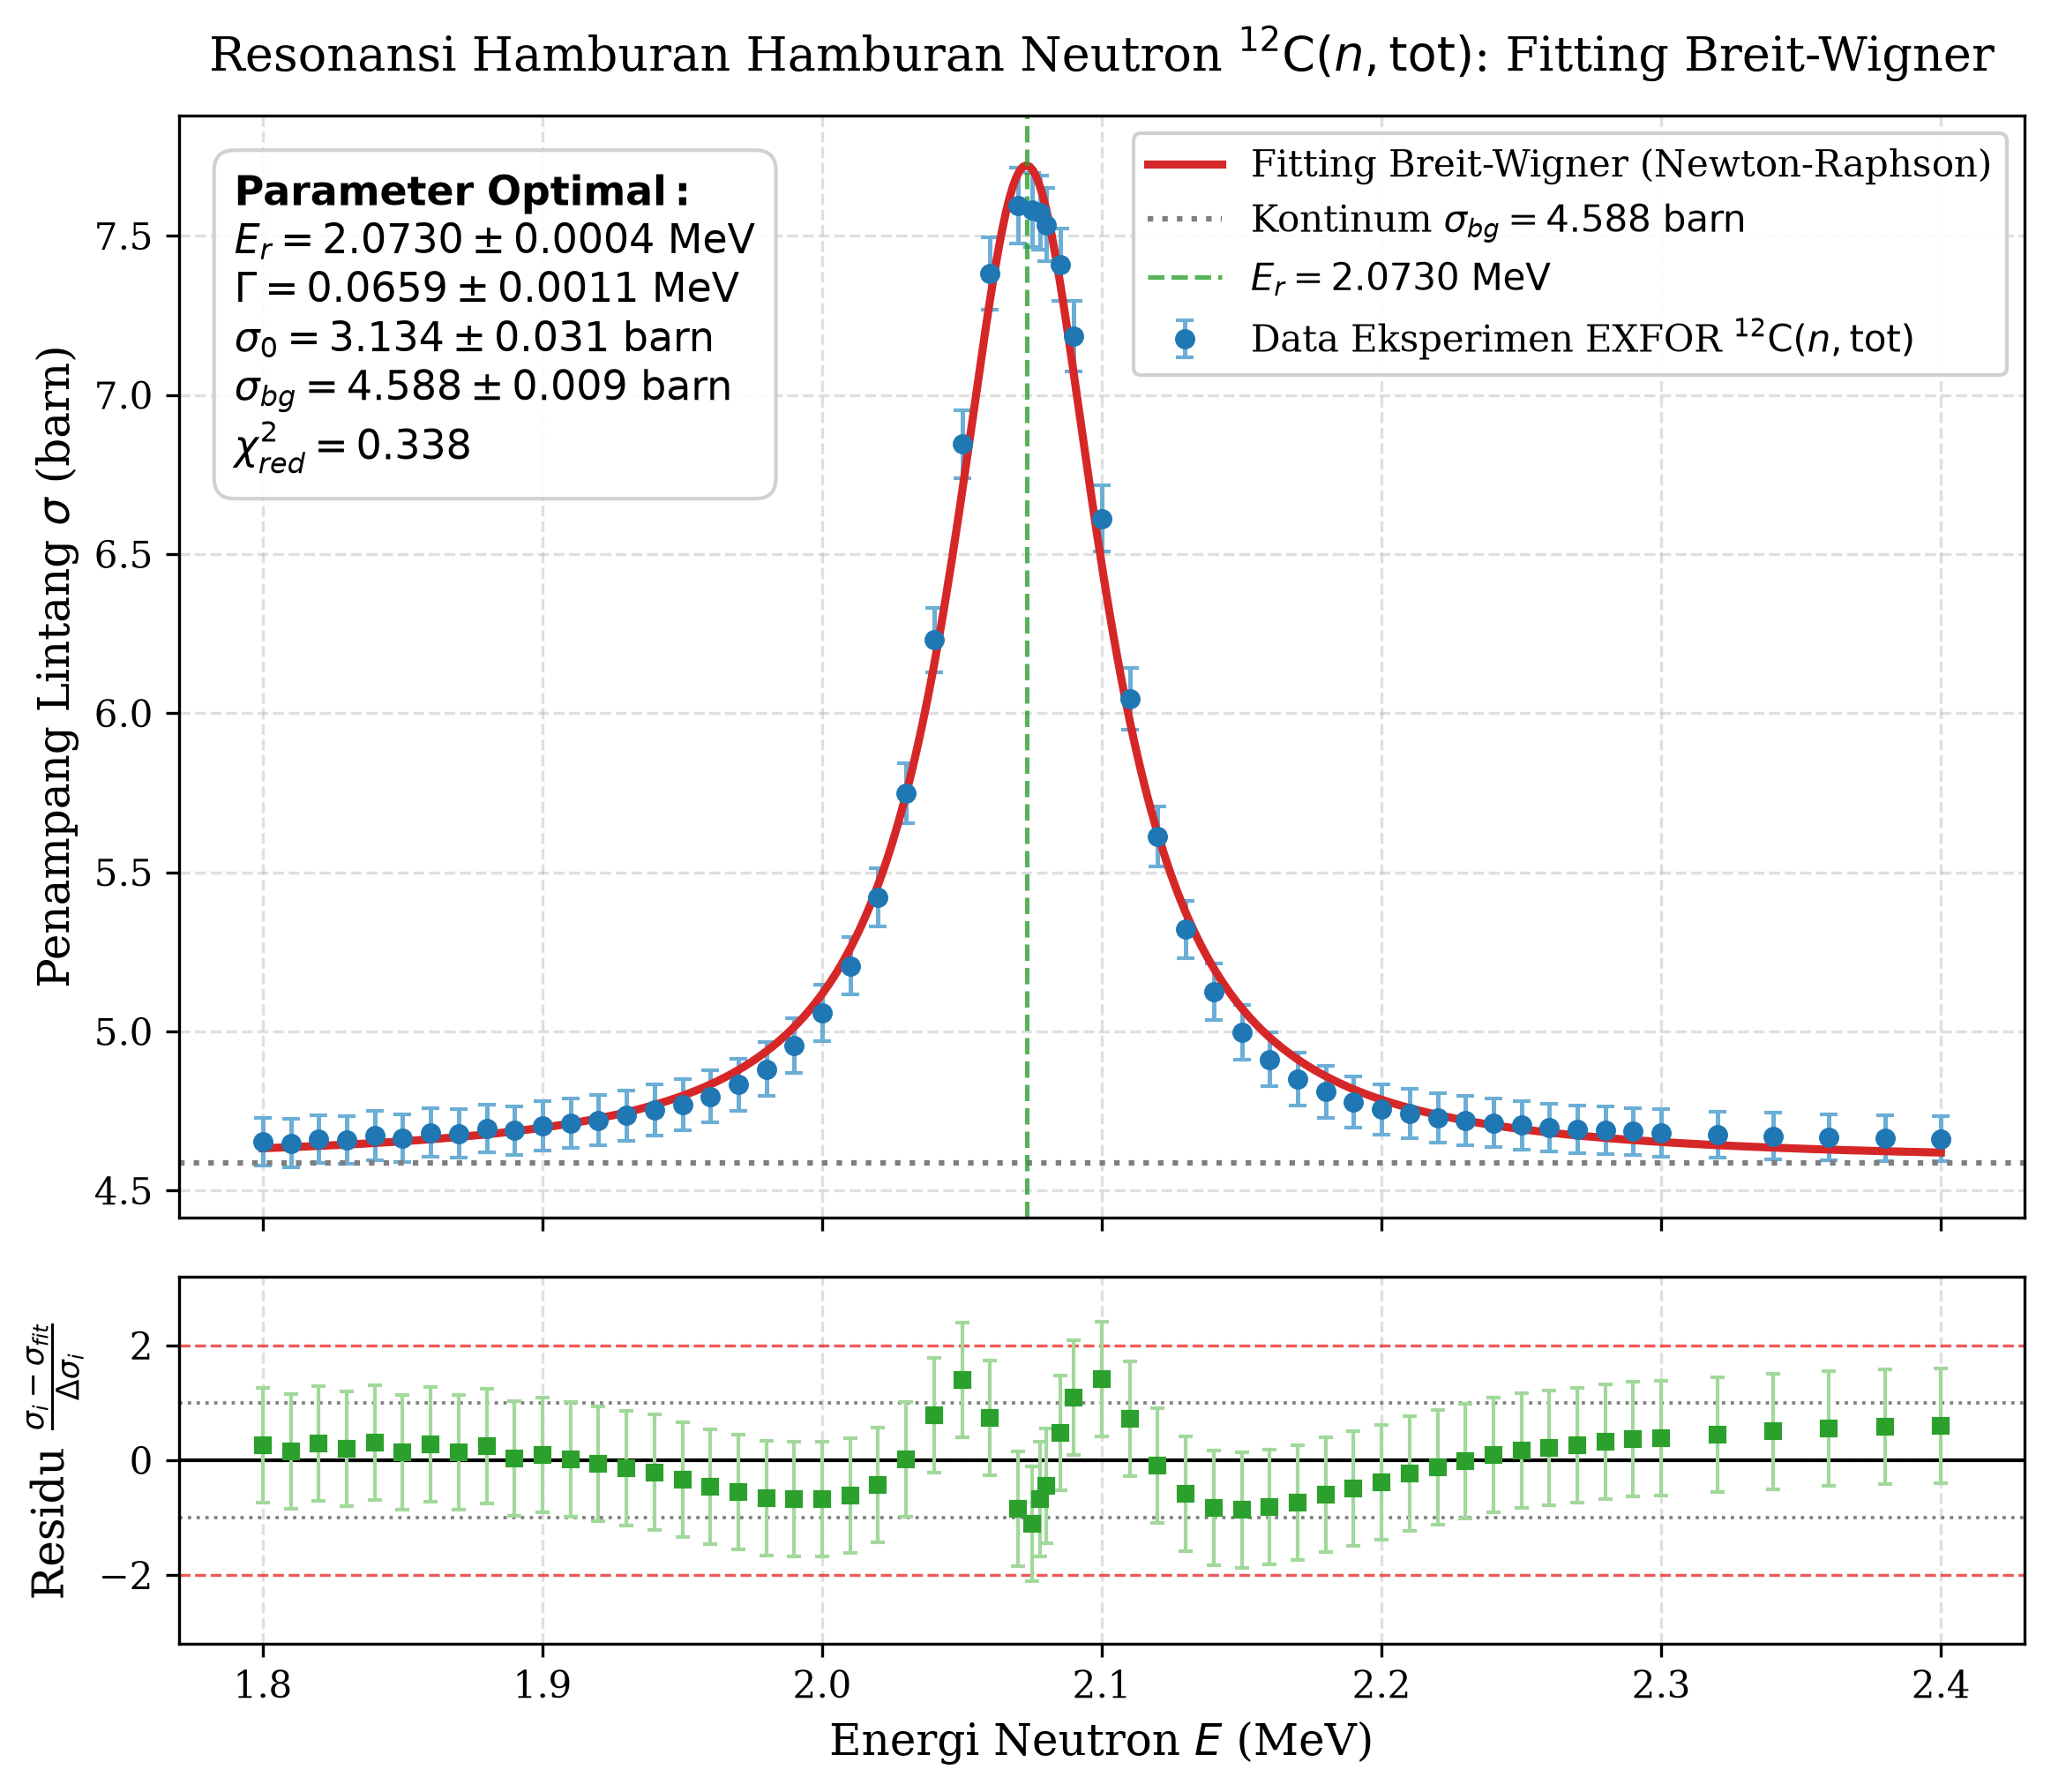
\includegraphics[width=0.88\textwidth,height=0.78\textheight,keepaspectratio]{resonance_fitting_plot.png}
	\end{center}
\end{frame}

% SLIDE 14: Profil Konvergensi
\begin{frame}{Profil Laju Konvergensi Kuadratik \& Kestabilan $\kappa(\mathbf{H})$}
	\begin{center}
		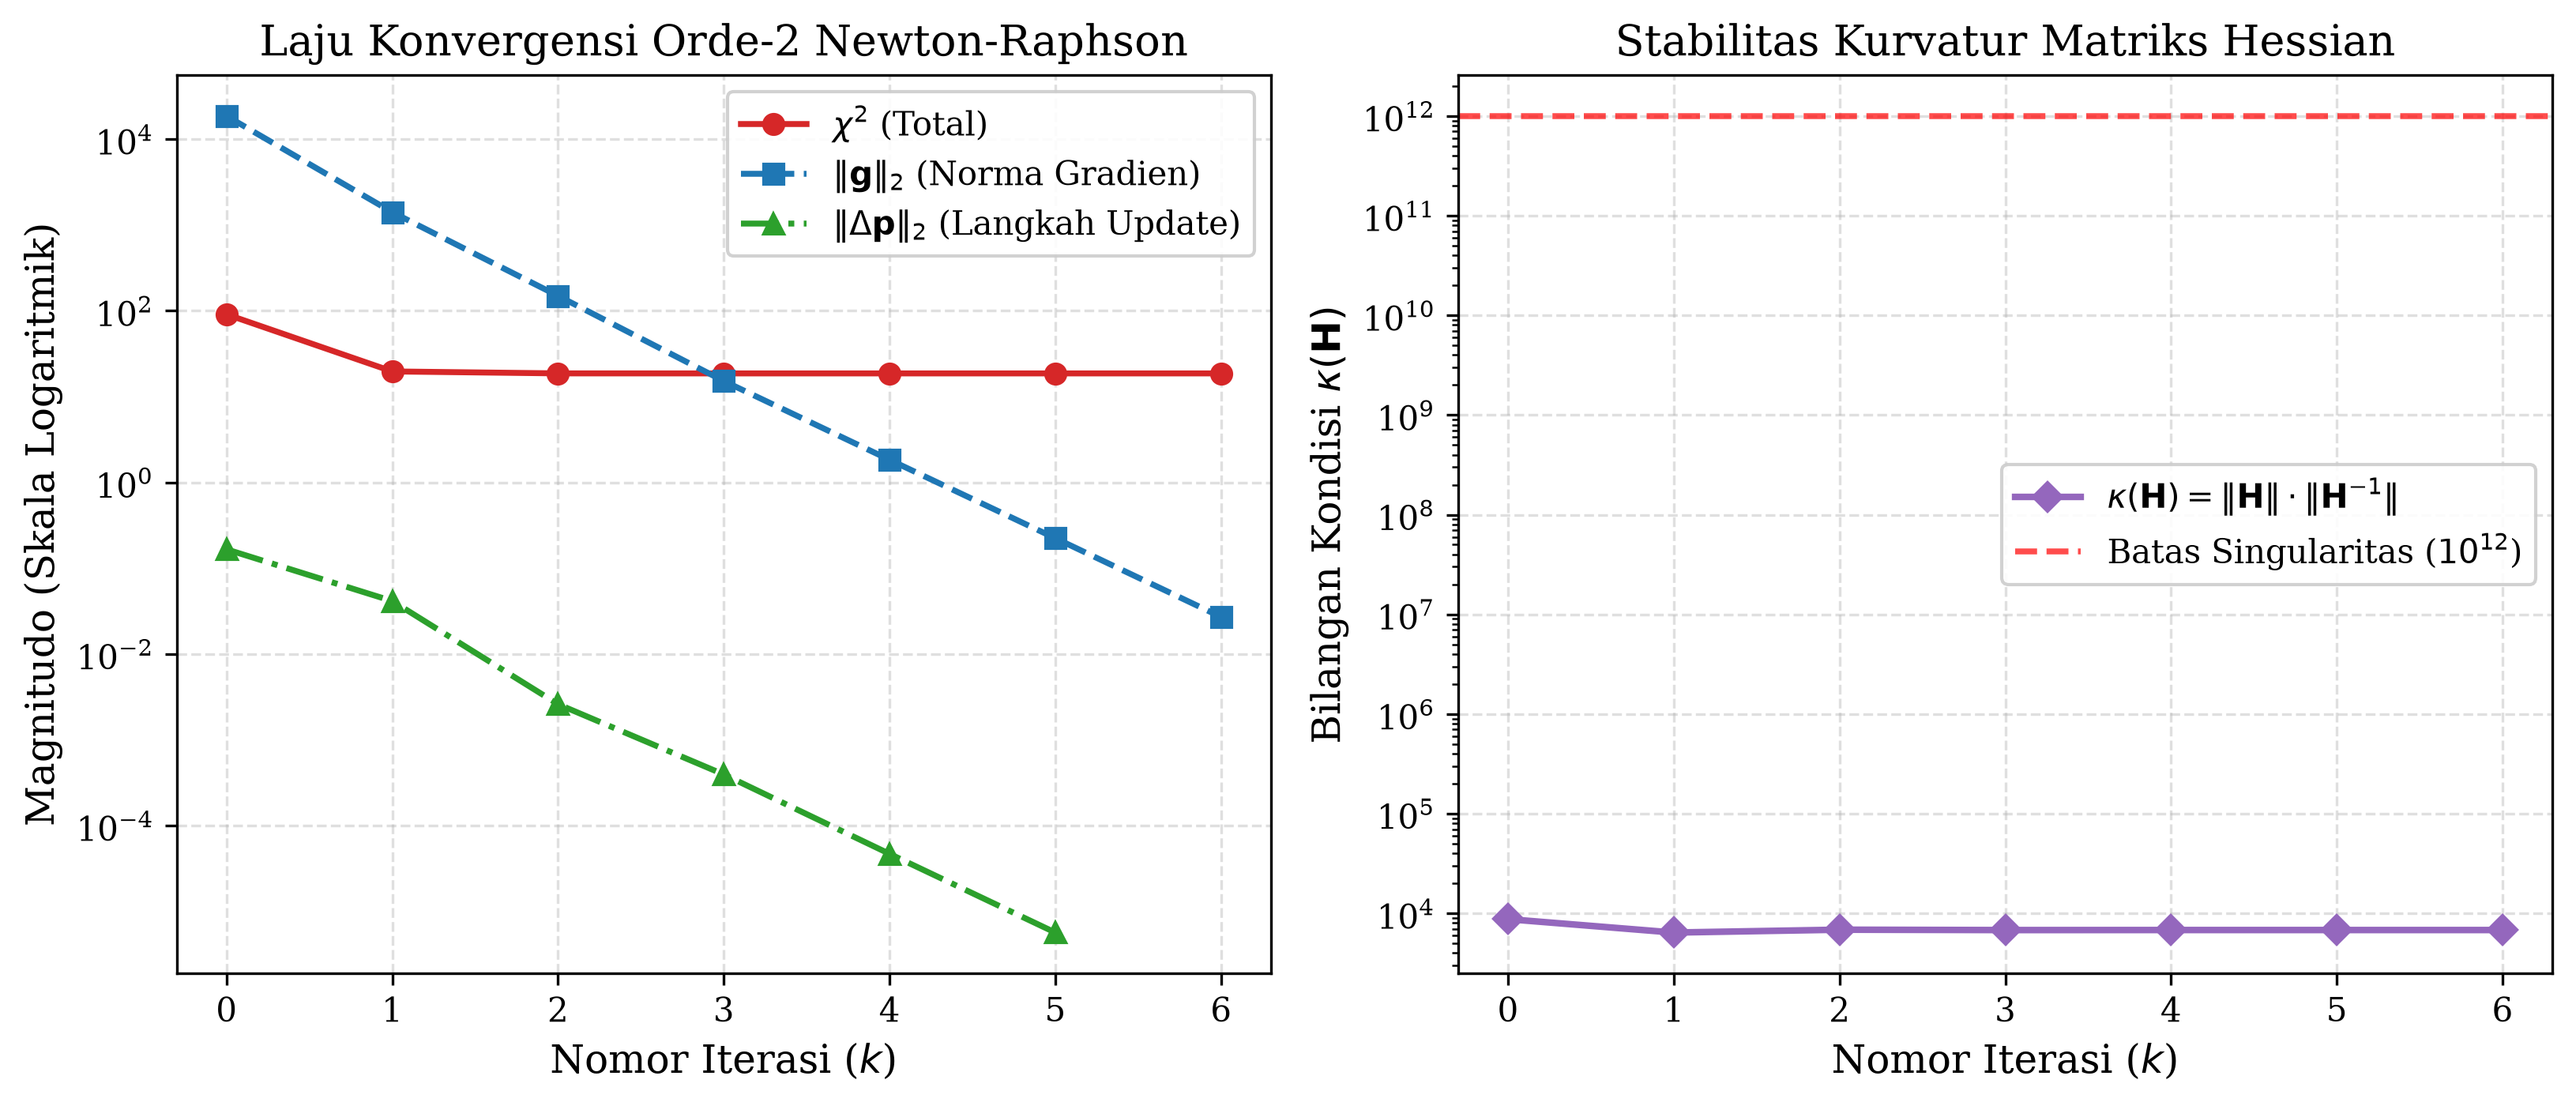
\includegraphics[width=0.88\textwidth,height=0.78\textheight,keepaspectratio]{convergence_metrics_plot.png}
	\end{center}
\end{frame}


% =============================================================
% SECTION 6: PEMBAHASAN
% =============================================================
\section{Pembahasan}

% SLIDE 15
\begin{frame}{Analisis Interdependensi Parameter: Matriks Korelasi}
	\begin{columns}[T]
		\begin{column}{0.5\textwidth}
			\begin{alertblock}{Anti-Korelasi Fisis $\Gamma$ vs $\sigma_0$ ($\rho = -0.4737$)}
				\small
				Bersumber dari hukum kekekalan integral luas penampang lintang resonansi:
				\begin{equation}
					\int_{-\infty}^{\infty} \sigma_{res}(E)\,dE = \frac{\pi}{2}\sigma_0\Gamma
				\end{equation}
				\footnotesize
				Jika $\sigma_0$ turun, $\Gamma$ naik untuk mempertahankan luas area total yang terukur eksperimen (kekekalan fluks hamburan).
			\end{alertblock}
		\end{column}

		\begin{column}{0.5\textwidth}
			\begin{block}{Interpretasi Fisis Korelasi Lainnya}
				\small
				\begin{itemize}
					\item \textbf{$\Gamma$ vs $\sigma_{bg}$ ($\rho = -0.5754$):} Tumpang-tindih ekor Lorentzian dengan kontinum hamburan potensial pada sayap spektrum.
					\item \textbf{$E_r$ ortogonal ($|\rho| \le 0.18$):} Posisi puncak ditentukan murni oleh simetri data, bebas dari lebar dan amplitudo.
					\item Analisis kovariansi menggunakan $\mathbf{C} = 2[\mathbf{H}(\mathbf{p}^*)]^{-1}$ --- relasi asimptotik Cram\'{e}r-Rao.
				\end{itemize}
			\end{block}
		\end{column}
	\end{columns}
\end{frame}

% SLIDE 16
\begin{frame}{Uji Ketahanan Derau Monte Carlo}
	\begin{columns}[c]
		\begin{column}{0.55\textwidth}
			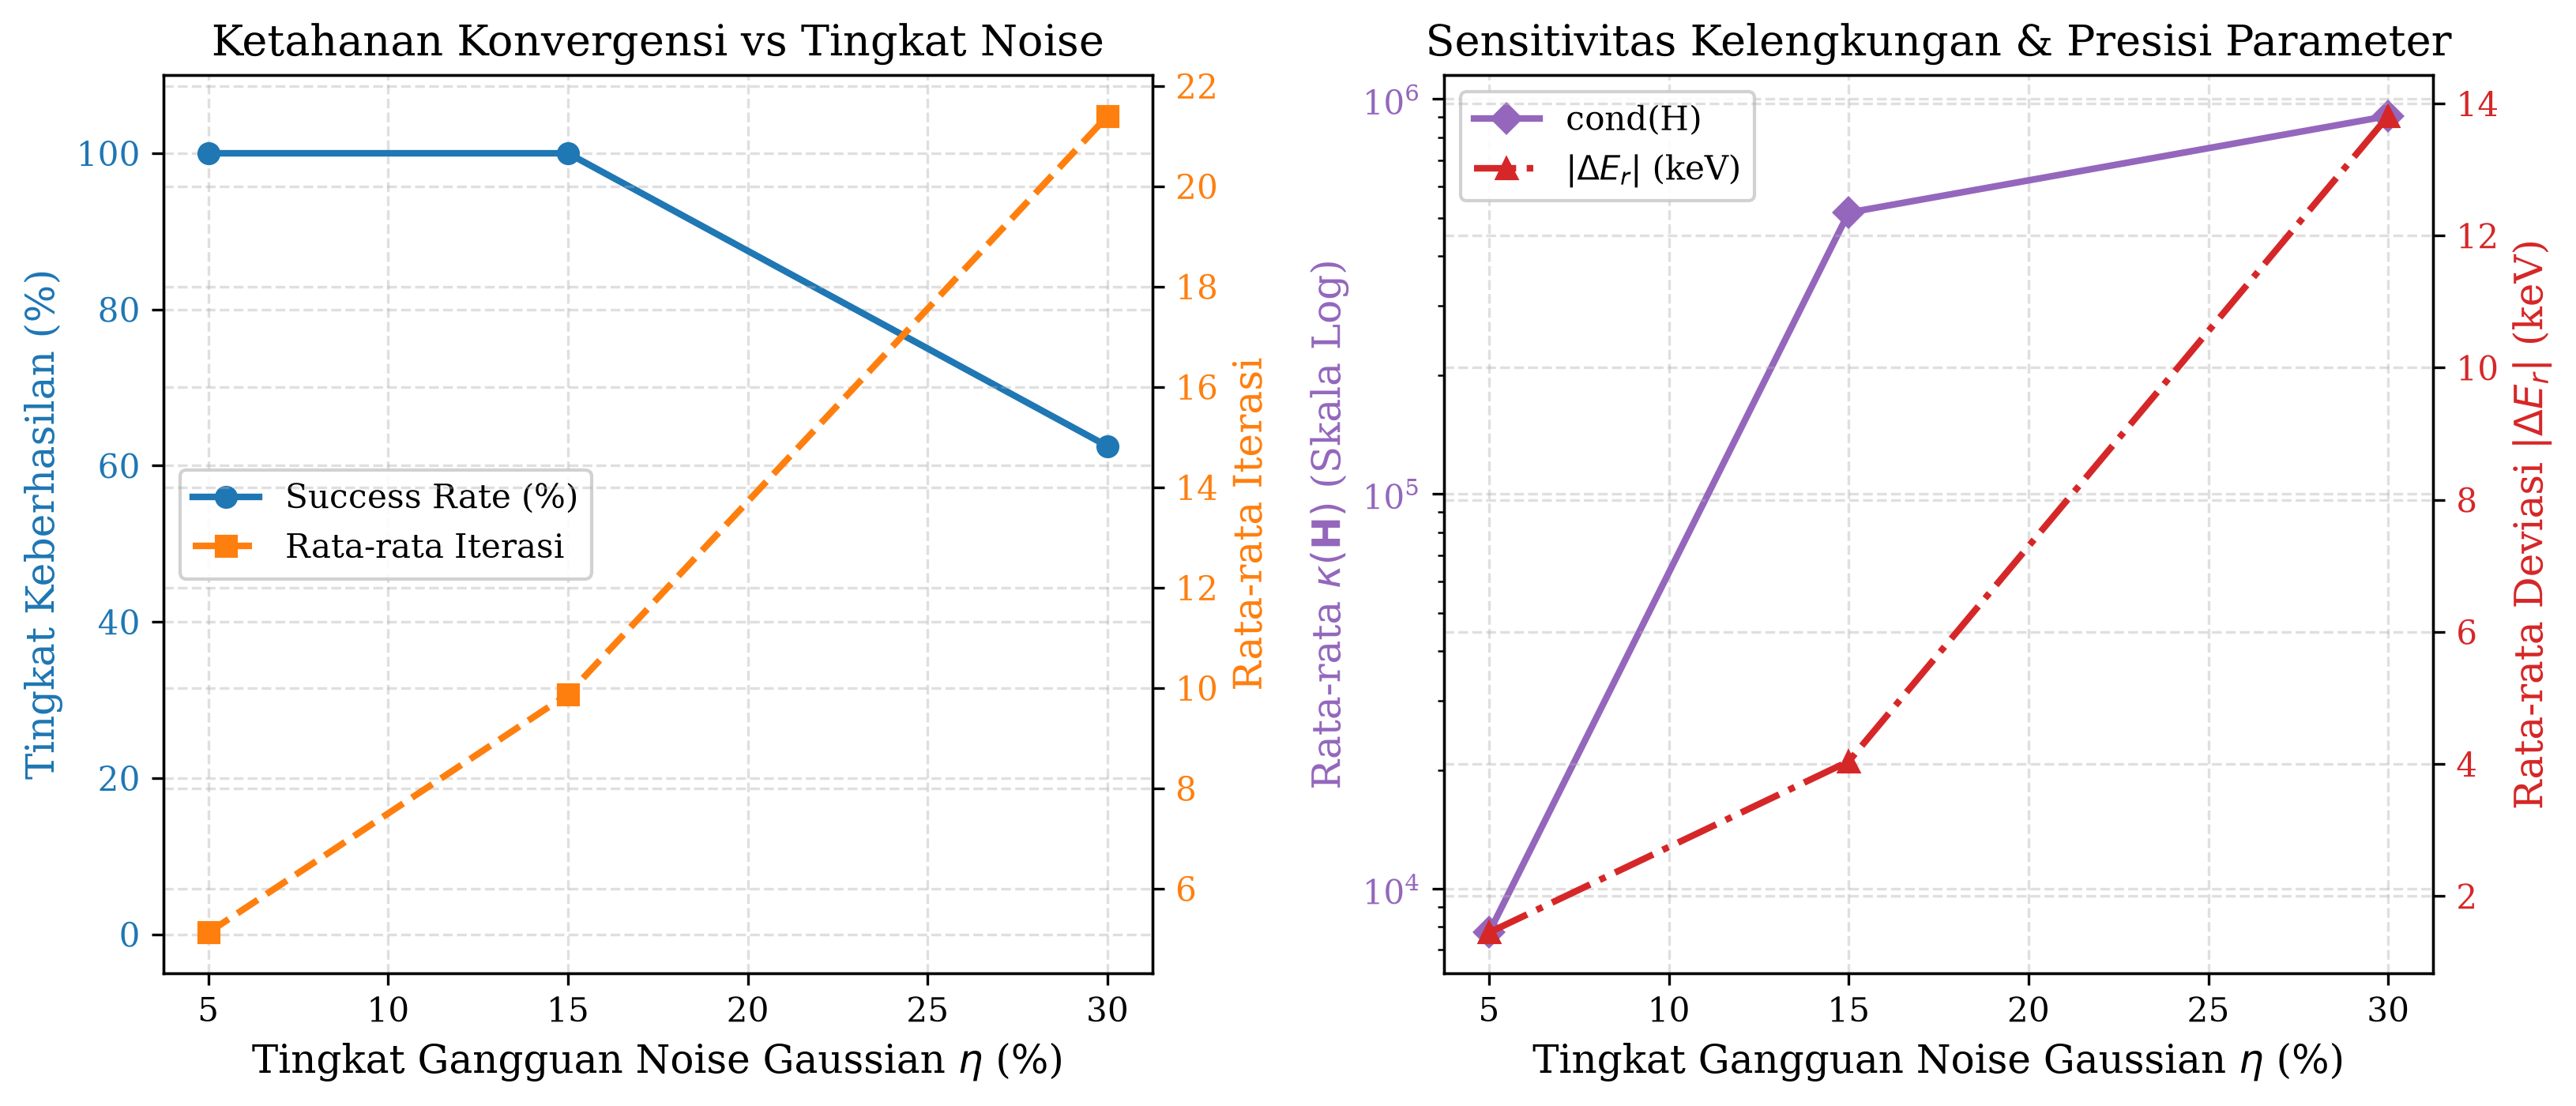
\includegraphics[width=\textwidth,height=0.68\textheight,keepaspectratio]{noise_stress_test_plot.png}
		\end{column}

		\begin{column}{0.45\textwidth}
			\begin{block}{Ringkasan Hasil Uji Ketahanan}
				\small
				\begin{table}
					\scriptsize
					\setlength{\tabcolsep}{3pt}
					\begin{tabular}{c c r r}
						\toprule
						$\eta$ & Laju Sukses & Iter. & $|\Delta E_r|$ \\
						\midrule
						$5\%$ & $100\%$ & 5.1 & $1.4\text{ keV}$ \\
						$15\%$ & $100\%$ & 8.5 & $4.7\text{ keV}$ \\
						$30\%$ & $60\%$ & 22.0 & $12.3\text{ keV}$ \\
						\bottomrule
					\end{tabular}
				\end{table}
				\footnotesize
				\begin{itemize}
					\item Tangguh $100\%$ hingga $\eta = 15\%$.
					\item Pada $\eta = 30\%$: $\kappa(\mathbf{H})$ melonjak $> 10^{15}$ pada kasus gagal, menandakan kehilangan sifat positif-definit lokal permukaan $\chi^2$.
					\item Regularisasi \textbf{Levenberg-Marquardt} direkomendasikan untuk derau ekstrem.
				\end{itemize}
			\end{block}
		\end{column}
	\end{columns}
\end{frame}

% SLIDE 17
\begin{frame}{Validasi Fisis terhadap Standar Internasional ENDF/B-VIII.0}
	\begin{columns}[T]
		\begin{column}{0.5\textwidth}
			\begin{exampleblock}{Komparasi Hasil vs Literatur Nuklir}
				\small
				\begin{table}
					\footnotesize
					\setlength{\tabcolsep}{4pt}
					\begin{tabular}{l r r}
						\toprule
						\textbf{Sumber} & $E_r$ (MeV) & Diskrepansi \\
						\midrule
						Hasil Komputasi & $2.073019$ & --- \\
						ENDF/B-VIII.0 CIELO & $2.078000$ & $4.98\text{ keV}$ \\
						\bottomrule
					\end{tabular}
				\end{table}
				\vspace{0.2cm}
				\textbf{Deviasi Relatif: $0.2397\%$} ($< 0.5\%$)
			\end{exampleblock}
		\end{column}

		\begin{column}{0.5\textwidth}
			\begin{block}{Interpretasi Diskrepansi Kecil}
				\small
				Selisih $4.98\text{ keV}$ berada dalam batas:
				\begin{itemize}
					\item Resolusi instrumen detektor TOF Karlsruhe (Cierjacks, 1968).
					\item Efek pergeseran fasa hamburan gelombang parsial $d$-wave dalam pembentukan $^{13}$C$^*$.
					\item Perbedaan metodologi analisis R-matriks ENDF vs. fitting SLBW langsung.
				\end{itemize}
				\footnotesize
				Keselarasan ini \textbf{membuktikan validitas fisis} model komputasi yang dikembangkan.
			\end{block}
		\end{column}
	\end{columns}
\end{frame}


% =============================================================
% SECTION 7: KESIMPULAN & SARAN
% =============================================================
\section{Kesimpulan \& Saran}

% SLIDE 18
\begin{frame}{Kesimpulan Komputasi \& Fisis}
	\begin{block}{7 Poin Kesimpulan Utama}
		\footnotesize
		\begin{enumerate}
			\item Model Breit-Wigner satu tingkat \textbf{berhasil diselesaikan} menggunakan Newton-Raphson multivariat berbasis Hessian Gauss-Newton analitik $\mathbf{H} = 2\mathbf{J}^T\mathbf{W}\mathbf{J}$.
			\item Konvergensi kuadratik penuh tercapai dalam \textbf{6 iterasi}, mereduksi $\chi^2$ dari $90.8117 \to 18.6064$.
			\item Parameter resonansi optimal: $E_r = 2.073019 \pm 0.000379\text{ MeV}$, $\Gamma = 0.065895 \pm 0.001148\text{ MeV}$, $\sigma_0 = 3.133715 \pm 0.030648\text{ barn}$, $\sigma_{bg} = 4.587609 \pm 0.008926\text{ barn}$.
			\item Model sangat representatif: $\chi^2_{red} = 0.3383$, residu terstandarisasi tersebar acak simetris pada $[-1.5, +1.5]$.
			\item Anti-korelasi $\Gamma$--$\sigma_0$ ($\rho = -0.4737$) mencerminkan kekekalan integral luas resonansi; $E_r$ bersifat independen ($|\rho| \le 0.18$).
			\item Algoritma $100\%$ tangguh terhadap derau hingga $\eta = 15\%$; pada $\eta = 30\%$ diperlukan regularisasi Levenberg-Marquardt.
			\item Validasi terhadap ENDF/B-VIII.0: diskrepansi hanya $0.2397\%$ ($4.98\text{ keV}$) --- \textbf{validitas fisis tinggi}.
		\end{enumerate}
	\end{block}
\end{frame}

% SLIDE 19
\begin{frame}{Saran Pengembangan Lanjutan}
	\begin{columns}[T]
		\begin{column}{0.5\textwidth}
			\begin{exampleblock}{Saran Metodologis Numerik}
				\small
				\begin{itemize}
					\item Implementasikan algoritma hibrida \textbf{Levenberg-Marquardt} ($\mathbf{H}_{LM} = \mathbf{H} + \lambda\,\mathrm{diag}(\mathbf{H})$) untuk data dengan $\mathrm{SNR} < 3$ atau derau $\eta > 30\%$.
					\item Tambahkan strategi \textit{line search} adaptif (Armijo/Wolfe) sebagai pengaman konvergensi global.
					\item Kembangkan estimasi ketidakpastian via \textit{Bootstrap Monte Carlo} untuk sampel data kecil.
				\end{itemize}
			\end{exampleblock}
		\end{column}

		\begin{column}{0.5\textwidth}
			\begin{block}{Saran Pemodelan Fisis Lanjutan}
				\small
				\begin{itemize}
					\item Perluasan ke formalisme \textbf{matriks-R multi-tingkat} (\textit{multilevel R-matrix}) untuk domain energi yang memuat banyak puncak resonansi tumpang-tindih.
					\item Masukkan koreksi \textbf{pelebaran Doppler termal} pada temperatur operasi reaktor.
					\item Penerapan pada isotop nuklir lain (misalnya $^{16}$O$(n,\text{tot})$, $^{56}$Fe$(n,\text{tot})$) dalam validasi pipeline komputasi.
				\end{itemize}
			\end{block}
		\end{column}
	\end{columns}
\end{frame}

% SLIDE 20: Daftar Pustaka
\begin{frame}{Daftar Pustaka Utama}
	\footnotesize
	\begin{itemize}
		\item Breit, G. \& Wigner, E. (1936). Capture of Slow Neutrons. \textit{Physical Review}, \textbf{49}(7), 519--531.
		\item Brown, D. A. et al. (2018). ENDF/B-VIII.0: The 8th Major Release of the Nuclear Reaction Data Library with CIELO-project Cross Sections. \textit{Nuclear Data Sheets}, \textbf{148}, 1--142.
		\item Cierjacks, S. et al. (1968). High Resolution Total Neutron Cross Sections for Carbon. KFK-1000, Kernforschungszentrum Karlsruhe.
		\item Danon, Y. et al. (2018). High-Resolution Neutron Transmission and Capture Measurements on Carbon. \textit{Nuclear Science and Engineering}, \textbf{189}(2), 120--138.
		\item Fr\"{o}hner, F. H. (2000). Evaluation and Analysis of Nuclear Resonance Data. \textit{Nuclear Science and Engineering}, \textbf{136}(3), 310--333.
		\item Hale, G. M. et al. (2014). R-matrix analyses of reactions in the $^{13}$C compound system. \textit{Physical Review C}, \textbf{90}(2), 024606.
		\item Nocedal, J. \& Wright, S. J. (2006). \textit{Numerical Optimization} (2nd ed.). Springer.
		\item Smith, D. L. (2004). Covariance Matrices for Nuclear Data. \textit{Annals of Nuclear Energy}, \textbf{31}, 1773--1799.
	\end{itemize}
\end{frame}

% SLIDE 21: Penutup
\centering
\begin{frame}[plain]
	\centering
	\vspace{1.5cm}
	
\includegraphics[width=2.2cm]{logo-unair.png} \\[0.4cm]
	{\Huge\textbf{\color{UnairBlue} TERIMA KASIH}} \\[0.5cm]
	{\large\textbf{Sesi Tanya Jawab \& Diskusi}} \\[0.8cm]
	\footnotesize
	\textcolor{DarkSlate}{Repositori Kode \& Data:}\\
	\texttt{\small https://github.com/xysilverberg/Neutron-Resonance-Breit-Wigner}
\end{frame}

\end{document}

